\documentclass[10pt,aspectratio=169]{beamer}

% All the boilerplate is in ccaslides.sty
% Note that this also pulls in a custom vogtwidebar.sty
\usepackage{ccaslides}

\author{Ji\v{r}\'i Lebl}

\institute[OSU]{%
Departemento pri Matematiko de Oklahoma {\^S}tata Universitato}

\title{Cultivating Complex Analysis:\\%
The exponential (1.2.1)\\%
Polar coordinates (1.2.2)}

\date{}

\begin{document}

\begin{frame}
\titlepage
\end{frame}

\begin{frame}
Define
the exponential $e^z$ for $z \in \C$ (using the real exponential and
sin/cos):
\begin{equation*}
\exp(z) =
e^{z} = 
e^{x+iy}
\overset{\text{def}}{=}
e^x e^{iy}
=
e^x\cos y + i e^x \sin y .
\end{equation*}

\medskip
\pause
Some immediate properties:
\begin{equation*}
e^{\bar{z}} = 
e^{x-iy} =
e^x\cos y - i e^x \sin y  = \overline{e^{z}} ,
\qquad
\sabs{e^{z}} = 
\sabs{e^{x+iy}} =
e^x .
\end{equation*}

\pause
\medskip

Graphs of the real and imaginary part:

\begin{center}
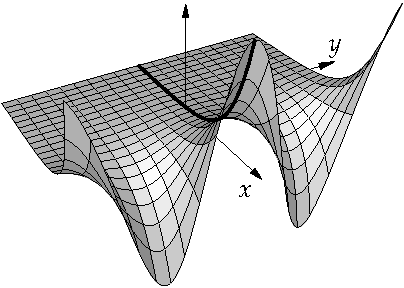
\includegraphics[width=2.0in]{../figures/realexp}
\qquad
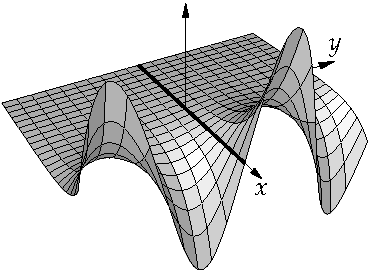
\includegraphics[width=2.0in]{../figures/imagexp}
\end{center}

\end{frame}

\begin{frame}
\begin{proposition}
For any two complex numbers $z,w \in \C$,
$
e^{z+w} = e^z e^w .
$
\end{proposition}

Proof is an exercise (requires trig identities).

\medskip
\pause
\textbf{Remark:}  $e^z$ is the unique continuous
function on $\C$ that satisfies $e^{z+w} = e^z e^w$ and $e^1 = e$.

\pause
\medskip

\emph{Euler's formula} ($\theta \in \R$):
\begin{equation*}
e^{i\theta}
=
\cos \theta + i \sin \theta .
\end{equation*}
\pause
Meaning for $\theta \in \R$:
\begin{equation*}
\cos \theta = \Re e^{i\theta} = \frac{e^{i\theta}+e^{-i\theta}}{2} ,
\qquad
\sin \theta = \Im e^{i\theta} = \frac{e^{i\theta}-e^{-i\theta}}{2i} .
\end{equation*}

\pause
We define sin and cos for $z \in \C$ accordingly:
\begin{equation*}
\cos z \overset{\text{def}}{=} \frac{e^{iz}+e^{-iz}}{2} ,
\qquad
\sin z \overset{\text{def}}{=} \frac{e^{iz}-e^{-iz}}{2i} .
\end{equation*}

\end{frame}

\begin{frame}
$\C$ is just the plane, so we can use \emph{polar coordinates} for $z=x+iy$:
$x = r \cos \theta$ and $y= r \sin \theta$.

\medskip
\pause
Due to the Euler formula:
\begin{equation*}
z = r e^{i\theta} = r\cos \theta + i r\sin \theta  = x+iy .
\qquad \qquad \qquad \qquad \qquad \qquad \qquad \qquad
\end{equation*}

\vspace*{-0.5in}
\hspace*{3.5in}\subimport*{../figures/}{polarcoords.pdf_t}

\vspace*{-0.4in}

\pause

We call $re^{i \theta}$ the \emph{polar form}.

\pause
\medskip


$r = \sabs{z} = \sqrt{x^2+y^2}$ is the modulus.

\pause
\medskip

$\theta$ is called the \emph{argument}.

\end{frame}

\begin{frame}

Polar form is good for multiplication and powers:

\pause
\medskip

Suppose $z = r e^{i\theta}$ and $w = s e^{i \psi}$,
\pause
\begin{equation*}
zw =
r e^{i \theta} s e^{i \psi} = 
rs e^{i (\theta+ \psi)},
\qquad
\frac{1}{z} =
\frac{1}{r e^{i \theta}} =
\frac{1}{r} e^{-i \theta} ,
\qquad
z^n =
{\bigl(r e^{i \theta}\bigr)}^n =
r^n e^{i n\theta} .
\end{equation*}

\medskip
\pause

Multiplication rotates by the argument and scales by the modulus.

\pause
\medskip

Again note that $i = e^{i \pi / 2}$ is
rotation counterclockwise by $90$ degrees.

\pause
\medskip

The downside is that the polar form is terrible for addition.

\end{frame}

\end{document}
